\chapter{Canadian Open Neuroscience Platform (CONP)}

\label{CONP}

Previously, we explained two of popular data and tool sharing platforms, OpneNeuro and NITRC. In this chapter we explain the Canadian Open Neuroscience Platform, another tool and data sharing platform which includes all the datasets and analysis pipelines we employed in our project. The first section is about the architecture of CONP, the technologies which are used and how CONP guarantees the principles of Open Science. In the second chapter, we focused on the CONP web interface and its capabilities. 

I have contributed to the technical development of CONP web platform and implemented some features, also I am a co-author in CONP paper which is submitted to Scientific Data. Therefore, some of the figures or data in this chapter is derived from either the paper or the website of CONP.

\section{Architecture of CONP}
The Canadian Open Neuroscience Platform (CONP) provides an infrastructure for the promotion of open-science workflows and the sharing of neuroscience data. There are several open-source technologies integrated in CONP web portal to provide extensible distributed federation of datasets, unified search capabilities for data and software tools, the ability to run analyses either on High-Performance Computing (HPC) infrastructures or locally.


\begin{figure*}
    \centering
    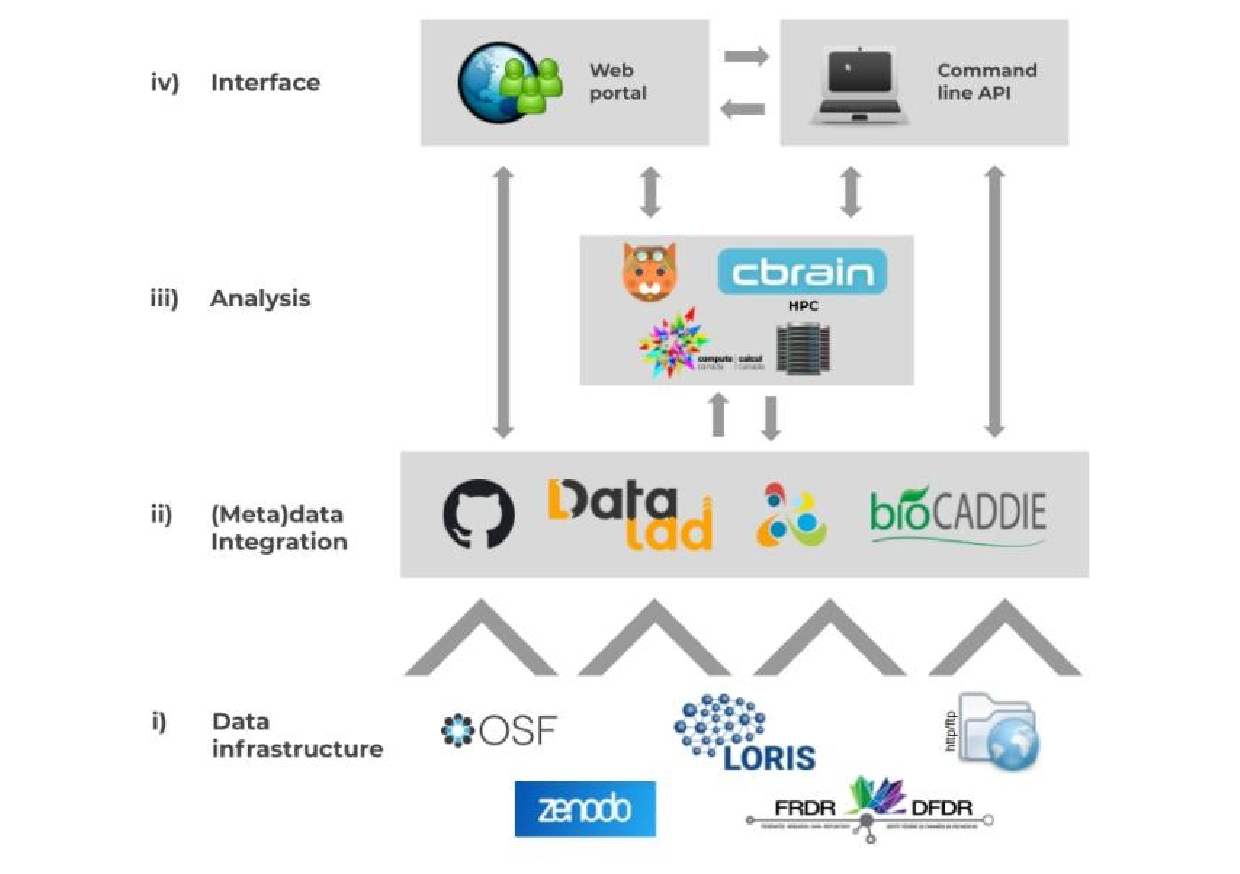
\includegraphics[width=\textwidth]{figures/CONP_figure.pdf}
    \caption{Architecture of the Canadian Open Neuroscience Platform. The platform is comprised of multiple tiers including:  i) independent data infrastructure; ii) Metadata integration across tools and datasets via standard models (Biocaddie DATS, Boutiques descriptors); iii) Data analysis on High-Performance Computing and; iv) Web and command-line interfaces. (The figure is captured from CONP paper\cite{CONP})}
    \label{fig:CONP_figure}
\end{figure*}

Figure~\ref{fig:CONP_figure} illustrates the architecture of CONP and since we focused on the available datasets and pipelines in CONP in our project, we explain the levels of this structure in following. 

\subsection{Data infrastructure}
CONP employes different distributed data repositories with different infrastructures, access control requirements, APIs, and licensing such as domain-agnostic datastores (OSF, Zenodo, FRDR-DFDR), specific brain imaging repositories (LORIS, XNAT, Brain-CODE), and the commonly used HTTP and FTP web protocols. Also, CONP is extensible to any repository which allows access via programmatic web-compatible interfaces.

\subsection{Data integration}
In the (meta)data integration layer, CONP leverages DataLad~\cite{} as a backend, GitHub~\cite{} to host the metadata, and enables uniform data search queries based on the Data Tags Suite model~\cite{}. Datalad is responsible for integration between datasets, it is a software library for managing Git repositories referencing the data through storing metadata, file URLs and hashes of data managed by git-annex. Therefore, a DataLad dataset does not contain the data themselves, the actual datasets remain stored remotely.

Also there is a crawling framework developed in CONP which manages the life cycle of DataLad datasets on GitHub. Using this crawler as web platform, users are able to upload datasets to the CONP without knowledge of Datalad or the GitHub workflow used in CONP. This crawler searches for CONP-tagged datasets and whenever a new dataset is found creates a Datalad dataset for that, and updates the Datalad dataset whenever a modification is detected in a dataset, and then updates the CONP forked GitHub repository. Also generates DATS file with minimal information for a dataset whenever the dataset does not have one.

CONP uses CircleCI as a dataset testing suit to periodically and continuously test if datasets are available, installable by Datalad, and if data are accessible by testing the download of a few files from the datasets. To detect possible issues, CircleCI repeats such tests every four hours for all available datasets in CONP and provides a continuous monitoring for them. Also, since CONP Datalad datasets are hosted in GitHub, the integration with CircleCi would be transparent and more feasible.

\subsection{Analysis and tools}
The analysis layer not only allows finding and downloading of tools, also allows directly integrating tools into workflows and their execution on High-Performance Computing (HPC) systems such as CBrain~\cite{}. All tools or pipelines available in CONP are described in Boutiques, "an open specification and software library for sharing tools according to the FAIR principles. Boutiques descriptors are JSON objects containing a specification of the tool input data, parameters, and output data. They link to a Docker or Singularity container image where the tool and all its dependencies are installed and configured for execution"~\cite{conppaper}. Tools described by boutiques  can be published, archived, and retrieved in the Zenodo and then assigned a DOI, which makes their archives permanently findable.

\subsection{Interface}
All the technologies and methods used in CONP are described as a web portal available at \url{http://portal.conp.ca} on which the users can search for, download and upload datasets, tools or pipelines, they are also able to lunch tools on their selected datasets using registered HPC systems such as CBrain without requiring advanced computing skills.  


 









\section{CONP web portal}

Canadian Open Neuroscience Platform (CONP) Portal is a web interface that facilitates open science for the neuroscience researchers by making datasets and tools globally accessible and shareable, the tutorial for the CONP portal is available at \url{https://portal.conp.ca/tutorial}. we will explain key features provided by the CONP portal is explained in the following. 

\subsection{Analytics}
A Dashboard that provides the key analytics that summarizes the  contents of the portal and introductory information, available at \url{https://portal.conp.ca/analytics}. All the data available in Analytics page will be updated automatically whenever there are updates in the number of uploaded dataset or pipeline, downloads, views and other statistics. One of the most important summarized contents in the Analytics page is about the available datasets and tool/pipelines in CONP.

\begin{figure*}[ht]
  \centering
  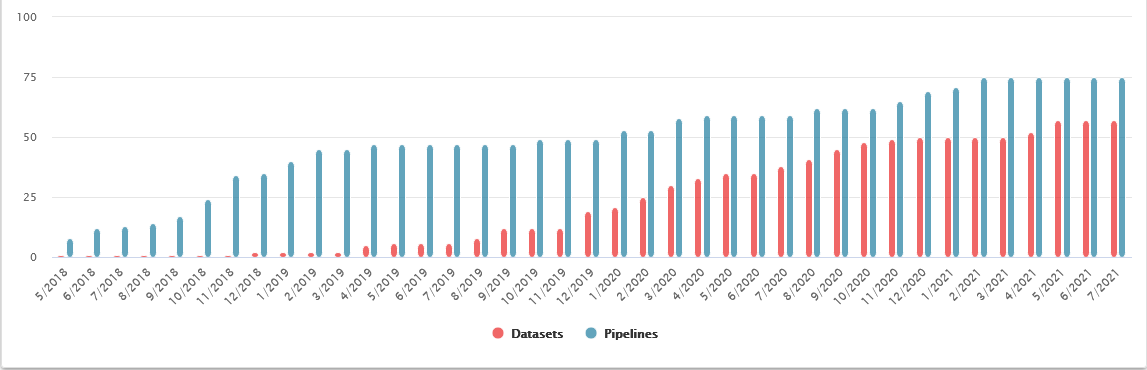
\includegraphics[width=\textwidth,height=\textheight,keepaspectratio]{figures/PipeDataTime.png}
  \caption{Cumulative number of datasets and pipelines. \\(Figure is copied form CONP portal at \url{https://portal.conp.ca/analytics})}
  \label{fig:cumulative}
  \end{figure*}

The number of pipelines and datasets has been increased in the last three years, see Figure~\ref{fig:cumulative}. At the beginning there has been only one dataset and eight pipelines in May 2018. There has been a marked rise in the number of datasets started in the end of 2019.
There are currently 57 datasets, as of July 2021, which are mostly neuroimaging and also transcriptomics, genomics, and other related data modalities. Most of these datasets are derived from neuroscience research institutes, a full list can be found here"~\url{https://portal.conp.ca/search}. There is usually a list of keywords and modalities assigned to each dataset which describes the category of compatibility of the dataset, Figure~\ref{fig:dataset_keyword} illustrates these keywords for the available datasets that are mostly 'brain imaging', 'human pain' and 'mri'. 

\begin{figure*}
    \centering
    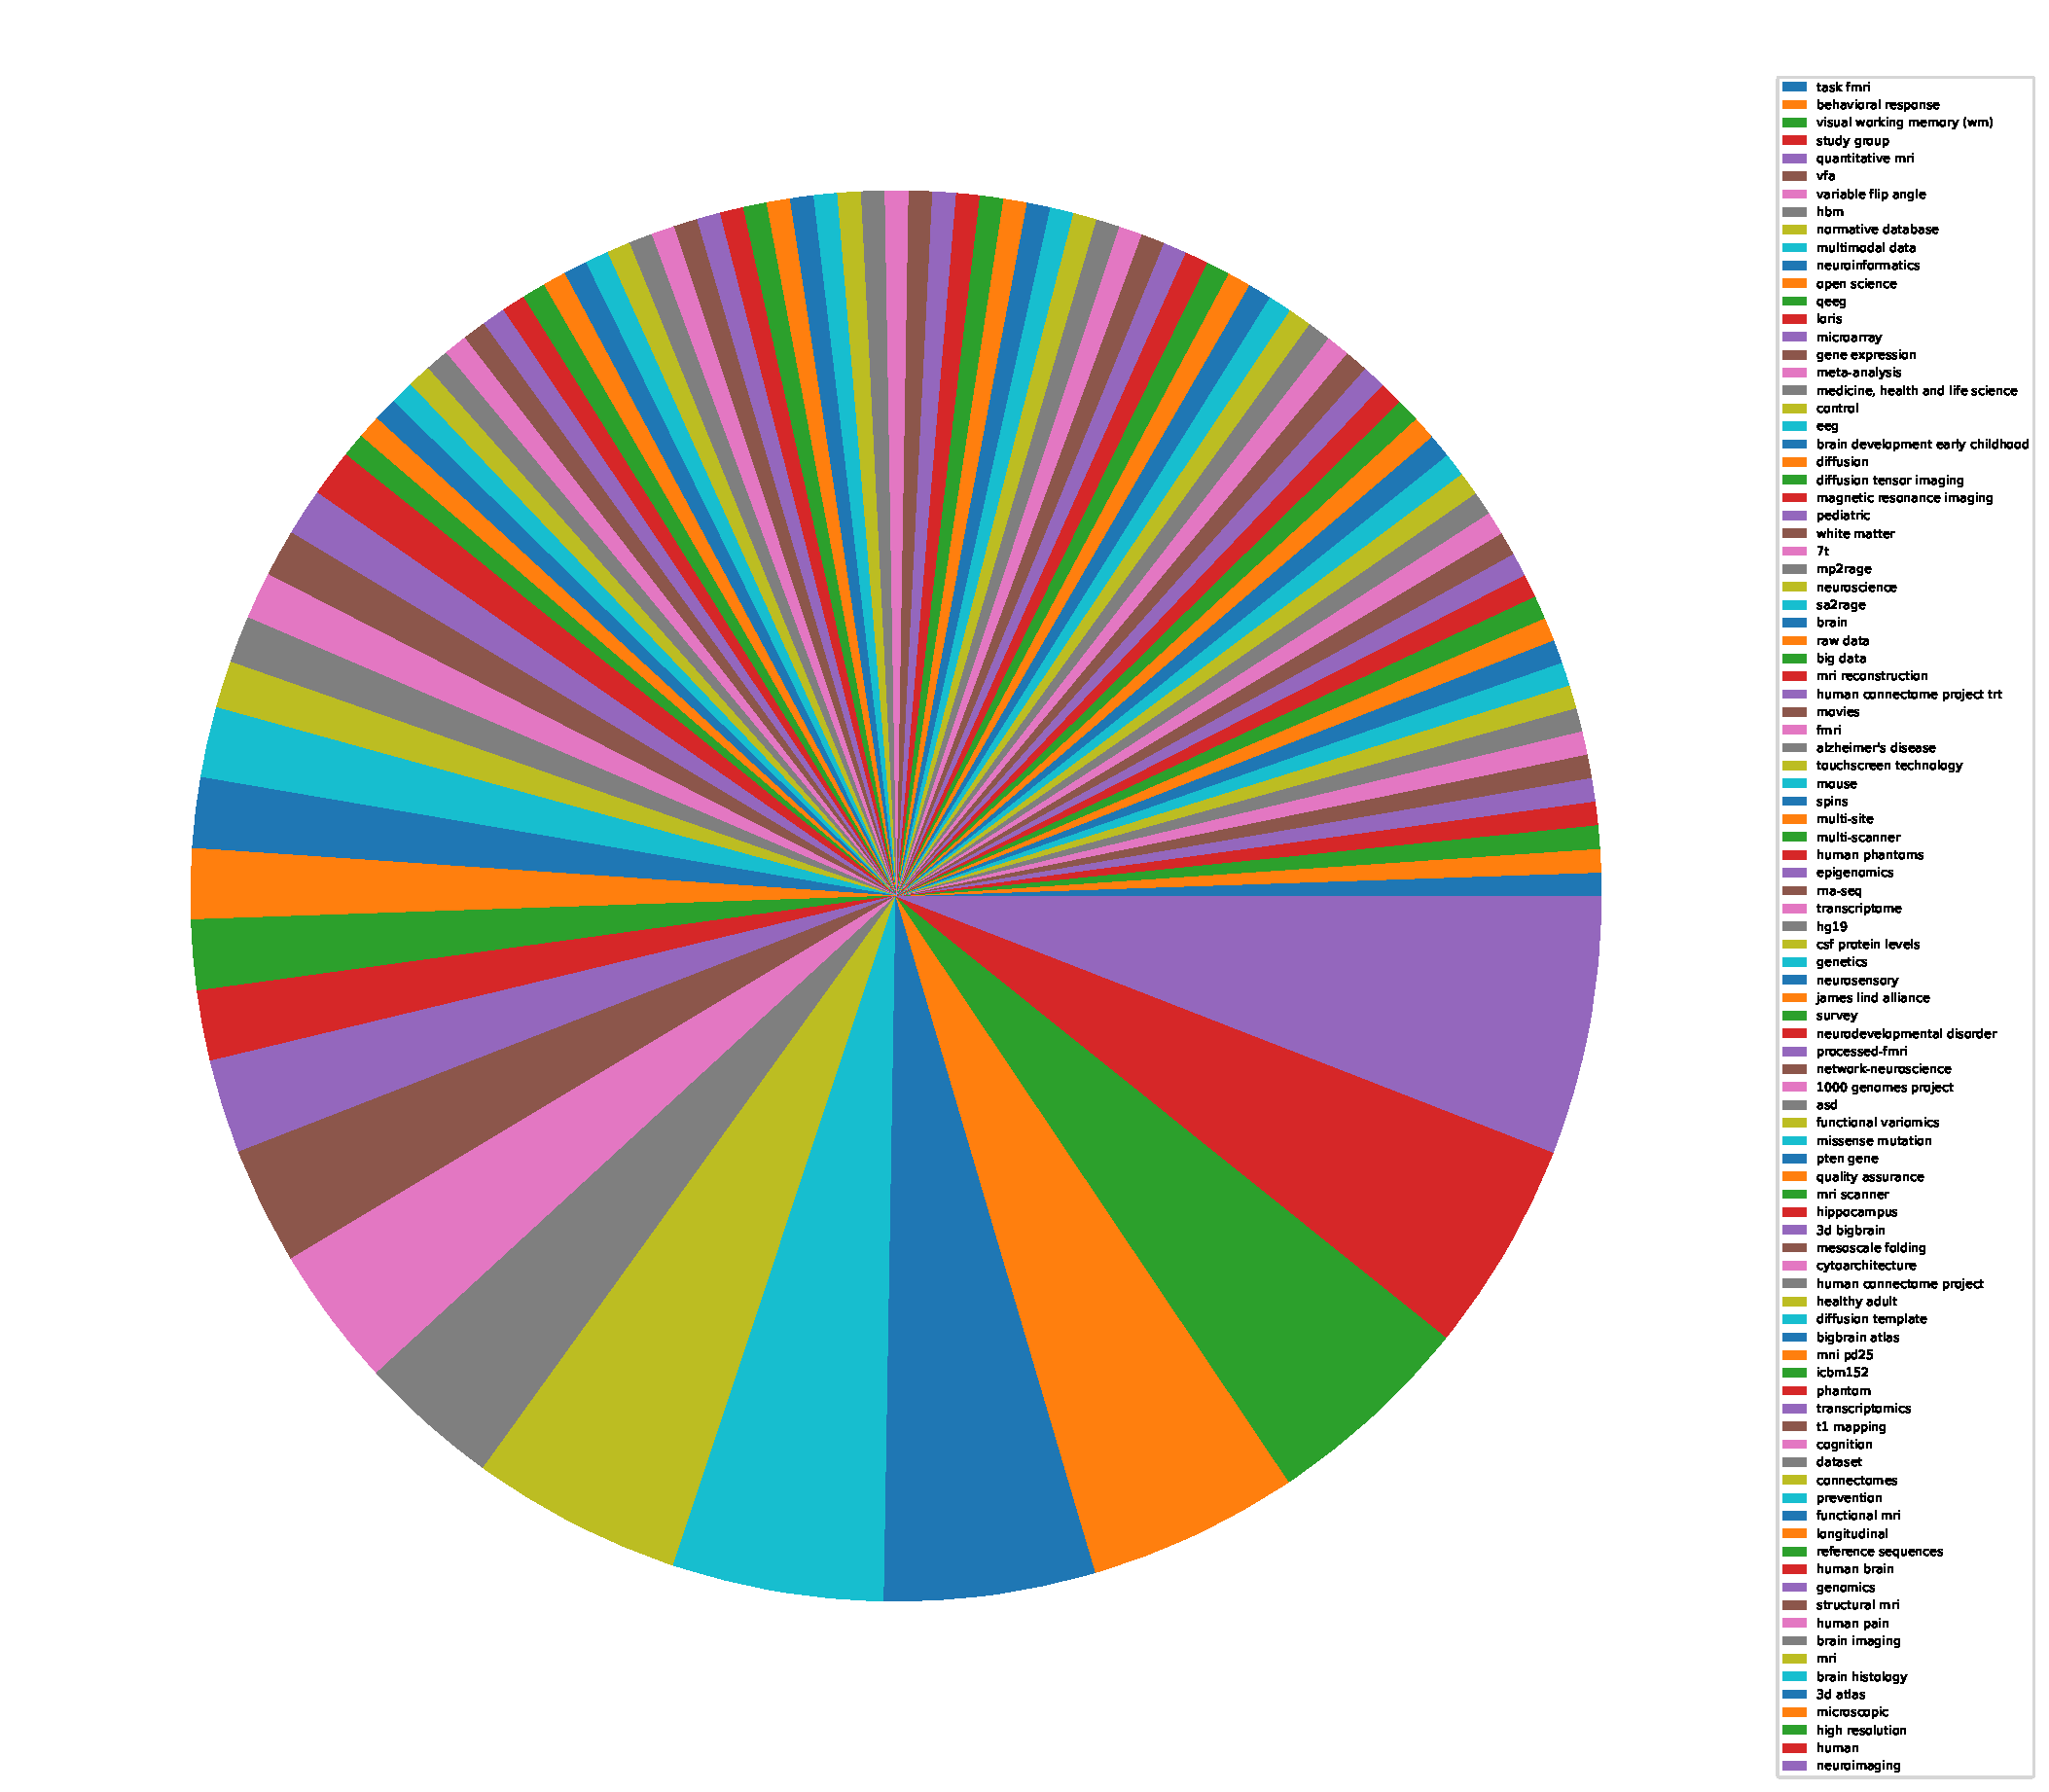
\includegraphics[width=\textwidth,height=\textheight,keepaspectratio]{figures/Datasets Keyword Pie Chart.pdf}
    \caption{Datasets' keywords\MM{will be pie chart}}
    \label{fig:dataset_keywords}
\end{figure*}

\begin{figure*}
    \centering
    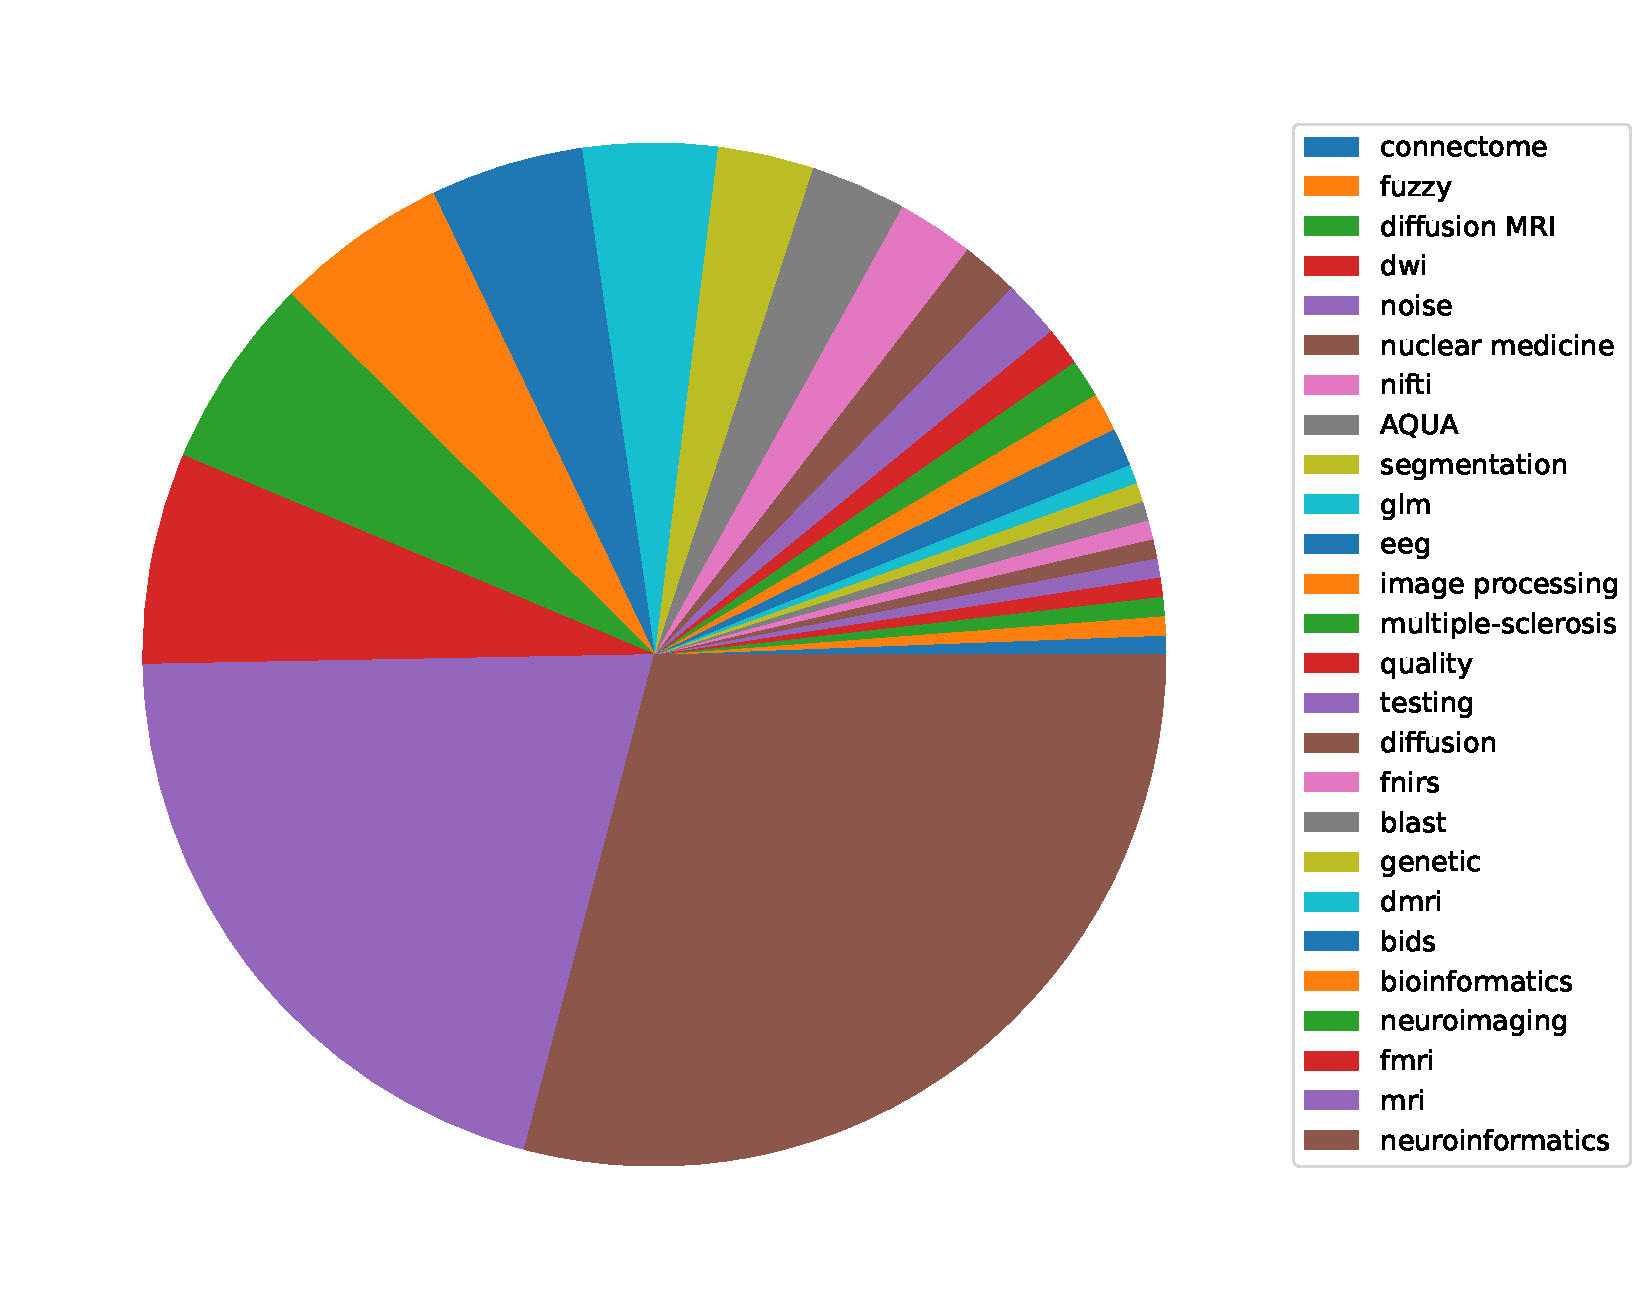
\includegraphics[width=\textwidth,height=\textheight,keepaspectratio]{figures/Pipelines Tag Pie Chart.pdf}
    \caption{Pipelines' tags \MM{will be pie chart}}
    \label{fig:pipelineTags}
\end{figure*}



Also, the number of pipelines has increased steadily in this period of time, currently there are 75 tools/pipelines which many of them come from neuroscience or genomics research institutes. There are some tags assigned to each tool/pipeline which describes its category of application, Figure~\ref{fig:pipelineTags}, which are mostly 'neuroinformatics' and 'mri'.

\begin{figure*}
\centering
\begin{subfigure}{\textwidth}  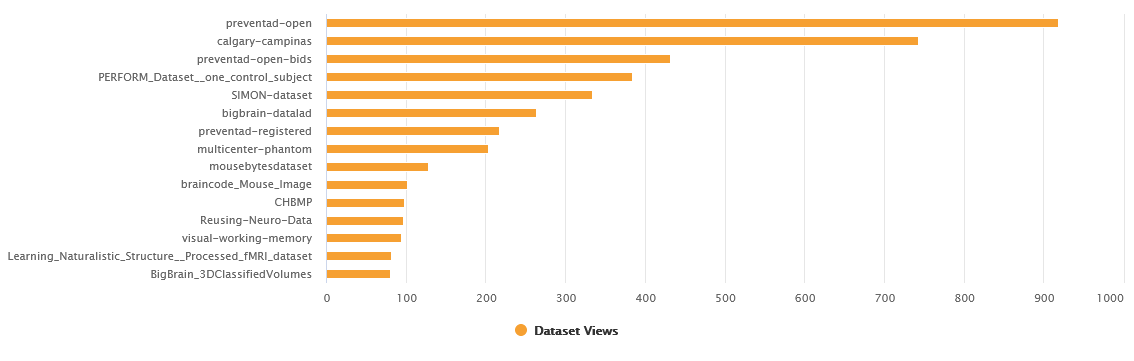
\includegraphics[width=\textwidth]{figures/mostV_datasets.png}
  \caption{Most Viewed Datasets}
  \label{fig:mostViewdDatasets}
\end{subfigure} \hfill
\begin{subfigure}{\textwidth}
  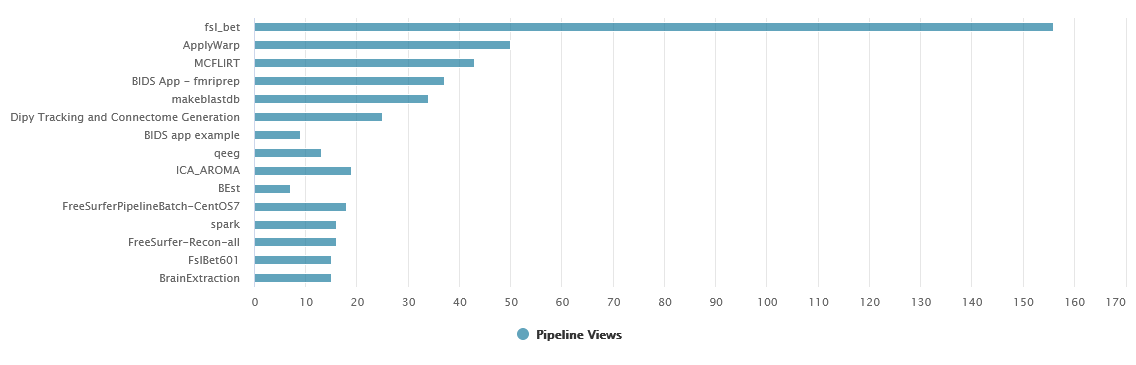
\includegraphics[width=\textwidth]{figures/mostV_pipelines.png}
  \caption{Most Viewed Pipelines}
  \label{fig:mostViewdPipelines}
\end{subfigure}
\caption{Most viewed datasets and pipelines through CONP portal \\(Figure is copied form CONP portal at \url{https://portal.conp.ca/analytics})}\label{fig:mostViewed}
\end{figure*}

Moreover, the Analytics page illustrates the most viewed datasets and pipelines, Figure~\ref{fig:mostViewed}, updating in a real-time manner which will be helpful for the new users and those who are willing to upload their own tool or dataset. For instance, fsl-bet which is the most viewed pipeline by far among all the pipelines, is also one of the most convenient ones to execute, it is fast and needs minimal requirements to execute, so would be ideal for the beginners in working with neuroimaging tools. Furthermore, when a tool/pipeline or dataset has most viewed means that there might be more resources and examples for that and the users can get more help in possible issues.


Another interesting outcome of showing the most popular tools/pipelines is that the pipeline developers can compare their own tool/pipeline with the most popular ones and get idea on how to improve their tool. Similarly, for the most viewed/popular datasets, not only the beginners might have more resources, examples and help and can choose those datasets to analyse, but also the dataset owners who aim at uploading their dataset can get ideas on the structure of the most popular dataset that might be helpful for them.


\subsection{Data Section}
In the Data section there is a filterable list of all datasets,
%the users are able to search for datasets based on specific features such as name of the dataset, data modalities
datasets can be filtered based on their modalities, file formats or the name of the dataset, see Figure~\ref{fig:search_data}. Also, there is an advance search option by which the user can specify some queries in SPARQL, this feature is still in experimental mode. Moreover, the datasets can be sorted based on a list of options such as number of files or subjects, latest update or size of dataset, to help users in finding the relevant dataset easier.

\begin{figure*}[ht]
  \centering
  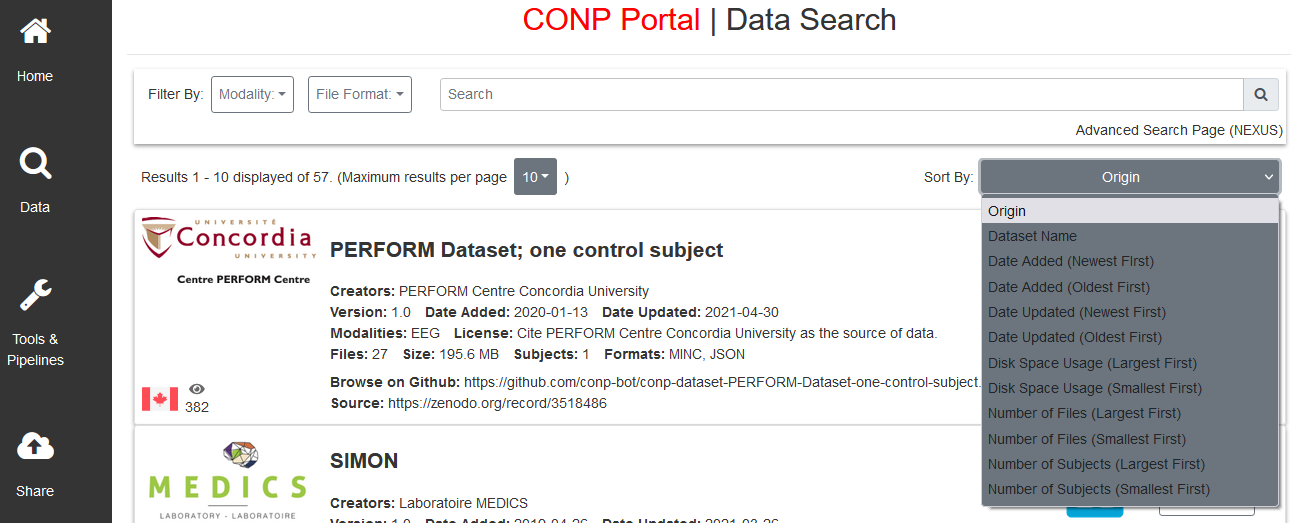
\includegraphics[width=\textwidth,height=\textheight,keepaspectratio]{figures/dataset_search.png}
  \caption{Dataset search engine. \\(Figure is copied form CONP portal at \url{https://portal.conp.ca/search})}
  \label{fig:search_data}
\end{figure*} 

For each dataset there might be also more options available, process on CBrain, downloading the metadata or the dataset itself~\ref{fig:data_card}, brows on Github and the source link of the dataset. To process a dataset on CBrain (if applicable), the user should have logged in to their account on CBrain and then they will be provided with a list of tools from which they can select to analyse the candidate dataset. They will also be able to set parameters for the candidate dataset and pipeline. \MM{why only some datasets have cbrain process option?}

The metadata of a dataset is stored in a JSON file and is simply downloadable, however to download a dataset, there are two possible approaches, direct downloading and download using Datalad. For many of datasets available in CONP direct download from the portal might not be possible either because of the large size of the dataset or because it requires a third-party account to access the data. While, downloading by Datalad is often the more applicable approach in which the user needs to install the Datalad dataset and then download it, tutorials are available in each dataset page. 




%Moreover, after getting the result of their analysis on CBrain, they will be able to upload the results as a new dataset
\begin{figure*}[ht]
  \centering
  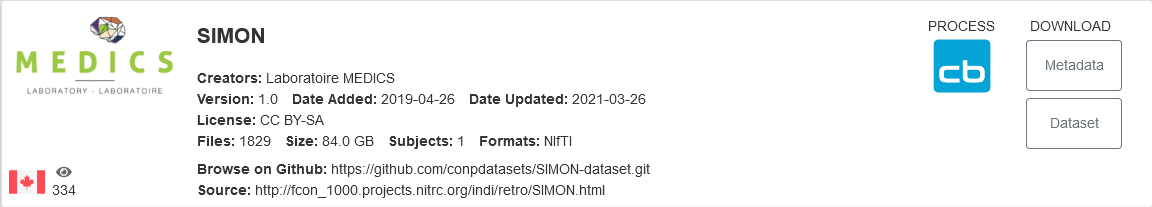
\includegraphics[width=\textwidth]{figures/dataCard.png}
  \caption{Dataset card. \\(Figure is copied form CONP portal at \url{https://portal.conp.ca/search})}
  \label{fig:data_card}
\end{figure*} 


\subsection{Tools and Pipelines section}
In the Tools and Pipelines section there is a filterable list of all available pipelines in CONP,
%the users are able to search for datasets based on specific features such as name of the dataset, data modalities
pipelines can be searched by their names or tags. For each pipeline, the number of views and downloads, its ID and the assigned tags are provided also users are able to sort the pipelines based on title, pipeline DOI or number of downloads~\ref{fig:pipeline_card}. Furthermore, for the pipelines which are registered in CBrain, it is possible to process that pipeline on CBrain with the data that the user should select on CBrain amon all registered datasets in CBRAIN~\ref{} and the parameters of the pipeline which should be set at execution process. 
\begin{figure*}[ht]
  \centering
  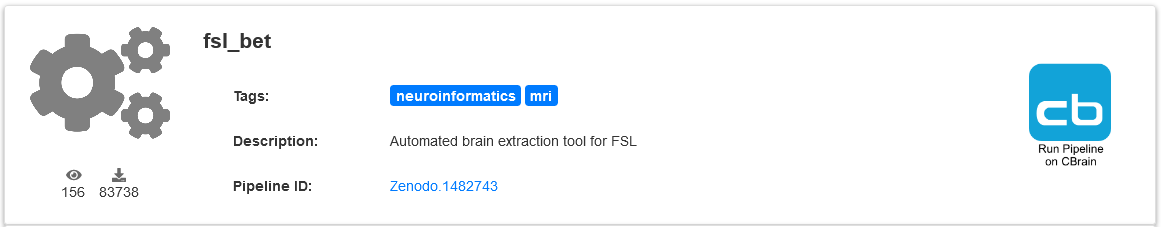
\includegraphics[width=\textwidth]{figures/pipelinecard.png}
  \caption{Pipeline card. \\(Figure is copied form CONP portal at \url{https://portal.conp.ca/pipelines})}
  \label{fig:pipeline_card}
\end{figure*} 

\begin{figure*}[ht]
  \centering
  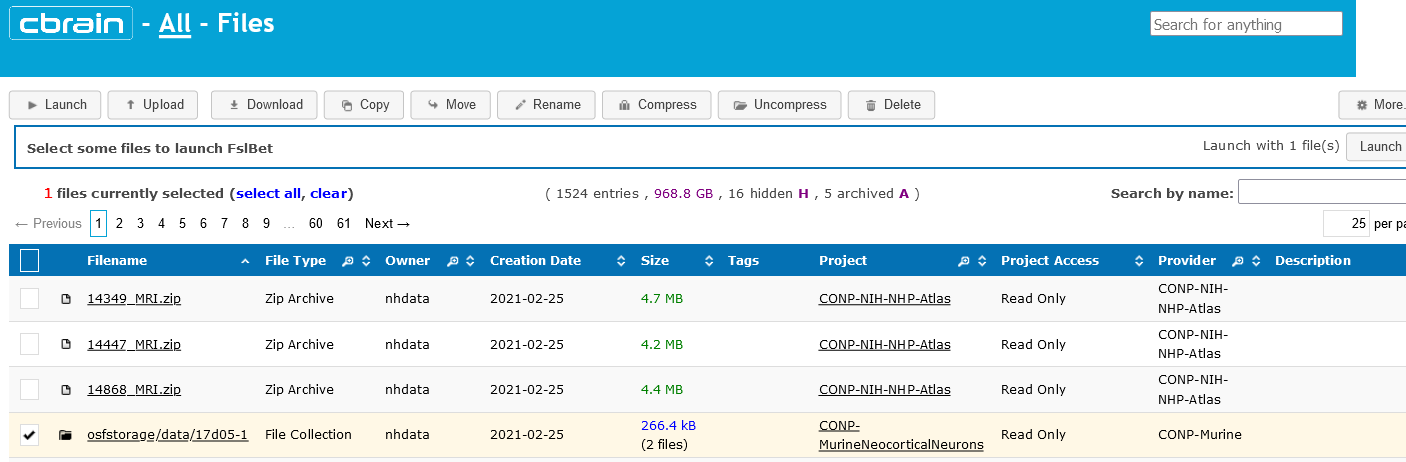
\includegraphics[width=\textwidth]{figures/CBRAIN.png}
  \caption{Data selection for processing a pipeline on CBRAIN }
  \label{fig:cbrainDataSelection}
\end{figure*} 

\begin{figure*}[ht]
  \centering
  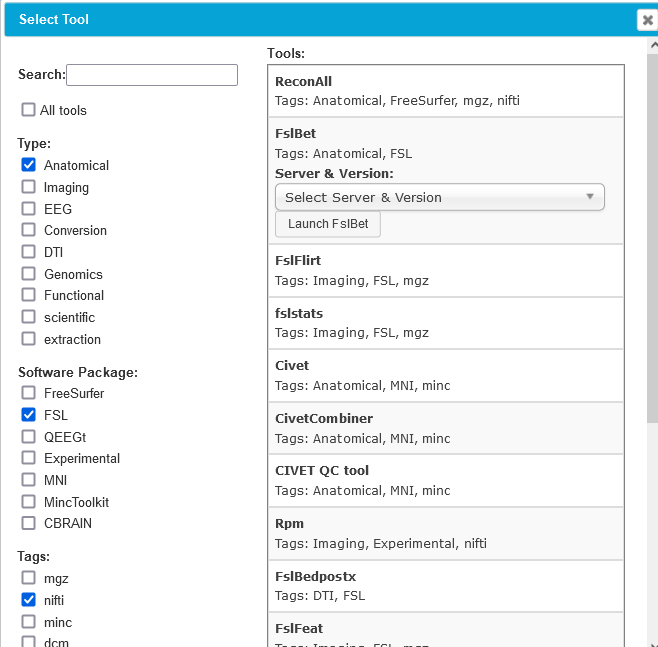
\includegraphics[width=\textwidth]{figures/CBRAIN_toolSelection.png}
  \caption{Pipeline settings for processing on CBRAIN}
  \label{fig:cbrainPipelineSettings}
\end{figure*} 

\subsection{Share section}
Through the Share section, the users are able to upload of data, tool/pipeline, and they also can edit the description of existing datasets or create a new description for their uploading dataset (each dataset should be described in the assigned DATS.json file).

For details and tutorials see \url{https://portal.conp.ca/share}

\subsubsection{Uploading data}

To upload their data, firstly the users should assign README and DATS.json files to the root directory of their dataset then they will be able to upload their dataset through Zenodo, OSF or Datalad. For uploading through Zenodo, for datasets larger than 50GB it is required to contact Zenodo support and request for larger dataset before uploading. Also for restricted access datasets they need to create Zenodo Personal Access Token and send it CONP Technical Steering Committee.


\subsubsection{Publish tool/pipeline}
The first step for publishing the tool/pipeline is to describe a command line for that and describe all possible options for their command line. Then they should create the JSON file which represents as the Boutiques tool descriptor (as mentioned before, all tools/pipelines in CONP are described in Boutiques), and requires a set of keys or properties which some of them are mandatory to be defined such as 'name' and 'input' and some are optional such as 'suggested-resources'. Then after finalizing the details about the parameters, input and output, and validating the tool descriptor, it would be ready to be published through Zenodo (See the full tutorial \href{https://nbviewer.jupyter.org/github/boutiques/tutorial/blob/master/notebooks/boutiques-tutorial.ipynb}{here}).  



\subsubsection{DATS editor}
There is a web interface available in CONP (\url{https://portal.conp.ca/dats-editor}) which helps users to generate the required DATS.json file describing their dataset and assign to that before uploading. They are also able to select the DATS file of an existing dataset on CONP, modify it using this interface and finally download the generated DATS.json file, then request CONP admin to accept that. 

\subsection{FAQ section}
In FAQ section, there are a set of questions and answer to support the user available at \url{https://portal.conp.ca/faq}


% The Portal internalizes the typical cycle of a research project, beginning with data acquisition, followed by data processing with published tools, and ultimately the publication of results with a link to the original dataset.

% The CONP Portal was built using technologies and best practices that make sharing easier and reproducible. DataLad and Git-Annex are used to track and index datasets, while Boutiques is used in conjunction with a container engine (e.g. Docker or Singularity) to ensure reproducibility of results. In addition, some pipelines can also be run using High Performance Computing (HPC) via links to the CBRAIN platform.





    % advanced dataset querying with Nexus
    % a dashboard representation of CONP Portal content and activities
